\documentclass[12pt, titlepage]{article}

\usepackage{amsmath, mathtools}

\usepackage[round]{natbib}
\usepackage{amsfonts}
\usepackage{amssymb}
\usepackage{graphicx}
\usepackage{colortbl}
\usepackage{xr}
\usepackage{hyperref}
\usepackage{longtable}
\usepackage{xfrac}
\usepackage{tabularx}
\usepackage{float}
\usepackage{siunitx}
\usepackage{booktabs}
\usepackage{multirow}
\usepackage[section]{placeins}
\usepackage{caption}
\usepackage{fullpage}
\externaldocument{../../SRS/SRS} 
\externaldocument{../MG/MG}
\hypersetup{
bookmarks=true,     % show bookmarks bar?
colorlinks=true,       % false: boxed links; true: colored links
linkcolor=red,          % color of internal links (change box color with linkbordercolor)
citecolor=blue,      % color of links to bibliography
filecolor=magenta,  % color of file links
urlcolor=cyan          % color of external links
}

\usepackage{array}
\newcommand{\rref}[1]{R\ref{#1}}
\newcommand{\ddref}[1]{DD\ref{#1}}
\newcommand{\mref}[1]{M\ref{#1}}
%% Comments

\usepackage{color}

\newif\ifcomments\commentstrue

\ifcomments
\newcommand{\authornote}[3]{\textcolor{#1}{[#3 ---#2]}}
\newcommand{\todo}[1]{\textcolor{red}{[TODO: #1]}}
\else
\newcommand{\authornote}[3]{}
\newcommand{\todo}[1]{}
\fi

\newcommand{\wss}[1]{\authornote{blue}{SS}{#1}}
\newcommand{\an}[1]{\authornote{magenta}{Author}{#1}}


\newcommand{\progname}{Program Name}

\begin{document}

\title{Module Interface Specification for Breaking Effect}

\author{Marshall Xiaoye Ma}

\date{\today}

\maketitle

\pagenumbering{roman}

\section{Revision History}

\begin{tabularx}{\textwidth}{p{3cm}p{2cm}X}
\toprule {\bf Date} & {\bf Version} & {\bf Notes}\\
\midrule
Date 2017-11-17 & 1.0 & New doc\\
\bottomrule
\end{tabularx}

~\newpage

\section{Symbols, Abbreviations and Acronyms}

See SRS Documentation at \url{https://github.com/MaXiaoye/cas741/blob/master/Doc/SRS/SRS.pdf}

\newpage

\tableofcontents

\newpage

\pagenumbering{arabic}

\section{Introduction}

The following document details the Module Interface Specifications for Breaking Effect.
 
Breaking effect presents how the pieces of an object move after it separates into parts with
suddenness or violence.

This project implements running time breaking effect in codes for 3-D models in unity3D without help from any similar plug-in. Including different shapes 3-D objects breaking based on physics and pieces interacting with the momentum provided by the breaking force. The breaking effect program simulates 3-D objects destruction process in vision by implementing scientific computing functions.

This project concentrates on calculation while
HCI or GUI are not important parts. Applied force is decided in codes in advance as input
and trace of motion is the output after calculation.

Complementary documents include the System Requirement Specifications
and Module Guide.  The full documentation and implementation can be
found at \url{https://github.com/MaXiaoye/cas741}.

\section{Notation}

The structure of the MIS for modules comes from \citet{HoffmanAndStrooper1995},
with the addition that template modules have been adapted from
\cite{GhezziEtAl2003}.  The mathematical notation comes from Chapter 3 of
\citet{HoffmanAndStrooper1995}.  For instance, the symbol := is used for a
multiple assignment statement and conditional rules follow the form $(c_1
\Rightarrow r_1 | c_2 \Rightarrow r_2 | ... | c_n \Rightarrow r_n )$.

The following table summarizes the primitive data types used by \progname. 

\begin{center}
\renewcommand{\arraystretch}{1.2}
\noindent 
\begin{tabular}{l l p{7.5cm}} 
\toprule 
\textbf{Data Type} & \textbf{Notation} & \textbf{Description}\\ 
\midrule
natural number & $\mathbb{N}$ & a number without a fractional component in [1, $\infty$) \\
real & $\mathbb{R}$ & any number in (-$\infty$, $\infty$)\\
String & String & represents sequences of characters.\\
Object & Object & A data structure to store attributes of input target object that provided by Unity3D.\\
PieceObject & PieceObj & A data structure to store attributes of pieces that generated as intermediate steps.\\
\bottomrule
\end{tabular} 
\end{center}

\noindent
The specification of \progname \ uses some derived data types: sequences, strings, and
tuples. Sequences are lists filled with elements of the same data type. Strings
are sequences of characters. Tuples contain a list of values, potentially of
different types. In addition, \progname \ uses functions, which
are defined by the data types of their inputs and outputs. Local functions are
described by giving their type signature followed by their specification.

\section{Module Decomposition}

The following table is taken directly from the Module Guide document for this project.

\begin{table}[h!]
	\centering
	\begin{tabular}{p{0.3\textwidth} p{0.6\textwidth}}
		\toprule
		\textbf{Level 1} & \textbf{Level 2}\\
		\midrule
		
		{Hardware-Hiding Module} & ~ \\
		\midrule
		
		\multirow{7}{0.3\textwidth}{Behaviour-Hiding Module} & Input Module\\
		& Piece Object Module\\
		& Obtaining gravity center module\\
		& Angle calculation module\\
		& Displacement in the air calculation module\\
		& Displacement on the ground calculation module\\
		\midrule
		
		\multirow{3}{0.3\textwidth}{Software Decision Module} & Target Object Module\\
		& Object cutting module\\
		& Output Module\\
		\bottomrule
		
	\end{tabular}
	\caption{Module Hierarchy}
	\label{TblMH}
\end{table}

\begin{figure}[H]
	\centering
	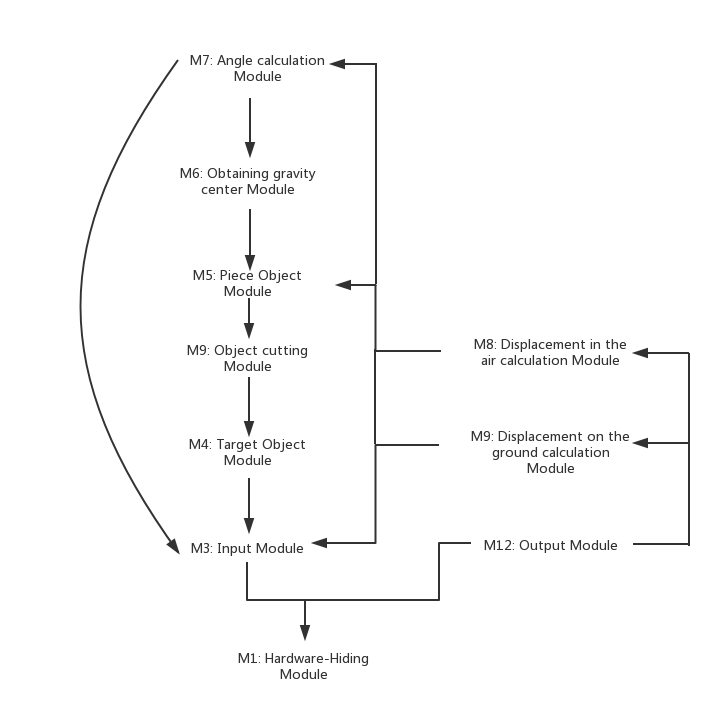
\includegraphics[width=0.7\textwidth]{./Figure1.png}
	\caption{Use hierarchy among modules}
	\label{FigUH}
\end{figure}

~\newpage

\section{MIS of Input Module(\mref{mIF})} 

This module collect verifies input from user and store in corresponding variables. Include position of target object, explosion level, coefficient of ground friction.

\subsection{Module}

InputModule

\subsection{Uses}

Hardware-Hiding Module (\mref{mHH})

\subsection{Syntax}



\subsubsection{Exported Access Programs}

\begin{center}
\begin{tabular}{p{2cm} p{4cm} p{4cm} p{2cm}}
\hline
\textbf{Name} & \textbf{In} & \textbf{Out} & \textbf{Exceptions} \\
\hline
$\mu_{k}$ &  $\mathbb{R}$ & - & InvalidInput\\
$E$ & $\mathbb{R}$ & - & InvalidInput\\
$TargetObj$ & $Object$ & - & InvalidInput\\
InputVerify() &  $\mathbb{R}^{2}; TargetObj$ & void & InvalidInput\\
\hline
\end{tabular}
\end{center}
\an{Object is a 3D model in Unity3D, which contains its position $(X,Y,Z)$. User needs provide a 3D model and attach the program to it.} 
\subsection{Semantics}

\subsubsection{State Variables}
None
\subsubsection{Access Routine Semantics}

\noindent InputVerifiy():
\begin{itemize}
\item transition: N/A
\item output: Exceptions or None.
\item exception:\an{Different kinds of exceptions for different invalid inputs.}\\
exc := ($\mu_{k}$ = null $\Rightarrow $ NoMuException)\\
exc := (E = null $\Rightarrow $ NoELvException)\\
exc := ($X,Y,Z \notin \mathbb{R} \vee (X,Y,Z \le -1000) \vee (X,Y,Z \ge 1000)$ $\Rightarrow $ InvalidCoorException)\\
exc := ($E \notin \mathbb{R} \vee (E \leq 0) \vee (E \geq 10)$ $\Rightarrow $ InvalidELvException)\\
exc := ($\mu_{k} \notin \mathbb{R} \vee (\mu_{k} \le 0) \vee (\mu_{k} \ge 1)$ $\Rightarrow $ InvalidMuException)\\
\end{itemize}

\section{MIS of target object module(\mref{mTO})}

Object class provided by platform

\subsection{Module}

TarObjModule

\subsection{Uses}

Input Module(\mref{mIF})

\subsection{Syntax}

\subsubsection{Exported Access Programs}

\begin{center}
	\begin{tabular}{p{2cm} p{4cm} p{4cm} p{2cm}}
		\hline
		\textbf{Name} & \textbf{In} & \textbf{Out} & \textbf{Exceptions} \\
		\hline
		$X$ & $\mathbb{R}$ & - & - \\
		$Y$ & $\mathbb{R}$ & - & - \\
		$Z$ & $\mathbb{R}$ & - & - \\
		position & $\mathbb{R}^{3}$ & - & - \\
		destory() & - & - & - \\
		\hline		
	\end{tabular}
\end{center}
$X,Y,Z$ are coordinates of object. position is 3D vector that contains $X,Y,Z$ while it is also considered as gravity center location of the object, destroy() function removes the object.
\subsection{Semantics}

\subsubsection{State Variables}

KeyCode.Space: Boolean.
This bool value indicates if key space is pressed on keyboard.

\subsubsection{Access Routine Semantics}

\noindent destroy():\\
\an{We assume the explosion happens when "space" is pressed. The target object is removed from scene at the same time.}
\begin{itemize}
	\item transition: target object $\rightarrow$ null
	\item output: None
	\item exception: None
\end{itemize}

\section{MIS of piece object module(\mref{mPO})}

Customize class for pieces that extend object class provided by platform. Pieces are generated after explosion happens to replace original target object from input.

\subsection{Module}

ObjCutModule

\subsection{Uses}

Input Module(\mref{mIF})

\subsection{Syntax}

\subsubsection{Exported Access Programs}

\begin{center}
	\begin{tabular}{p{2cm} p{4cm} p{4cm} p{2cm}}
		\hline
		\textbf{Name} & \textbf{In} & \textbf{Out} & \textbf{Exceptions} \\
		\hline
		Tag & String & - & - \\
		$x$ & $\mathbb{R}$ & - & - \\
		$y$ & $\mathbb{R}$ & - & - \\
		$z$ & $\mathbb{R}$ & - & - \\
		position & $\mathbb{R}^{3}$ & - & - \\
		onGround & Boolean & - & - \\
		$\theta_{1}$ & $\mathbb{R}$ & - & - \\
		$\theta_{2}$ & $\mathbb{R}$ & - & - \\
		Move() & Boolean & - & - \\
		Translate() & $\mathbb{R}^{3}$ & Visualization & - \\
		\hline
	\end{tabular}
\end{center}

\noindent Assumptions:\\
Tag, $x,y,z$ and position, Translate() are inheritated from parent class\\
\begin{itemize}
	\item Tag is string "piece" that indicates the object is an instance piece object.
	\item $x,y,z$ are coordinates of object.
	\item position is 3D vector that contains $x,y,z$.
	\item Translate() controls motion of the object.
	\item onGround indicates if the object is on the ground.
	\item $\theta_{1}, \theta_{2}$ are calculated and described in \mref{mAC}.
	\item  Move() controls motion of the object by calling Translate(). It check onGround firstly to make sure the object is in the air or on the ground. Based on value of bool variable onGround, that call and provide corresponding destination as input to Translate(). Destination to Translate() is calculated by \mref{mDC1} and \mref{mDC2}. \\
	\an{The definition of this class doesn't use \mref{mDC1} and \mref{mDC2} while result from \mref{mDC1} and \mref{mDC2} are only passed to function Move() that is called in \mref{mOM}. So I don't put \mref{mDC1} and \mref{mDC2} in Uses part.}
\end{itemize}

\subsection{Semantics}

\subsubsection{State Variables}

None

\subsubsection{Access Routine Semantics}

\noindent Move():
\begin{itemize}
	\item transition: None
	\item output: None
	\item exception: None
\end{itemize}

\noindent Translate():
\begin{itemize}
	\item transition: None
	\item output: Visualization
	\item exception: None
\end{itemize}

\section{MIS of acquiring pieces module (\mref{mOGC})} 

Call cutting function provided by Unity3D to split target object into pieces then do traversal to acquire all pieces. \an{Each piece is stored as an instance of class piece object defined in \mref{mPO}. Gravity center is position value in PieceObj}

\subsection{Module}

ObtainGCModule

\subsection{Uses}

Input Module(\mref{mIF})\\
Object cutting module(\mref{mOC})\\

\subsection{Syntax}

\subsubsection{Exported Access Programs}

\begin{center}
	\begin{tabular}{p{2cm} p{4cm} p{4cm} p{2cm}}
		\hline
		\textbf{Name} & \textbf{In} & \textbf{Out} & \textbf{Exceptions} \\
		\hline
		Traverse() & PieceObj;$\mathbb{R}$ & List of PieceObj & -\\
		\hline
		
	\end{tabular}
\end{center}

\subsection{Semantics}

\subsubsection{State Variables}
None
\subsubsection{Access Routine Semantics}

\noindent Traverse():\\
This function do a Traverse to store all piece objects into a list by filtering tags with "piece". Piece objects are initialed after target object is cutted. \an{tags for piece objects are defined in \mref{mPO}}
\begin{itemize}
	\item transition: None
	\item output: List of PieceObj 
	\item exception: None
\end{itemize}

\section{MIS of Angle calculation module(\mref{mAC})} 
Calculate the angle between initial speed $v_{0}$ and horizontal $\theta_{1}$. Calculate the angle between $x$ axiom and projection on horizontal of initial speed $\theta_{2}$. \an{$\theta_{1}$ and $\theta_{2}$ are values of each PieceObj}
\subsection{Module}

AngleCalModule

\subsection{Uses}

Input Module(\mref{mIF})\\
Obtaining gravity center module (\mref{mOGC})

\subsection{Syntax}

\subsubsection{Exported Access Programs}

\begin{center}
	\begin{tabular}{p{2cm} p{4cm} p{4cm} p{2cm}}
		\hline
		\textbf{Name} & \textbf{In} & \textbf{Out} & \textbf{Exceptions} \\
		\hline
		AngleSH() & $\mathbb{R}$;PieceObj & $\mathbb{R}$ & - \\
		AngleXV() & $\mathbb{R}$;PieceObj & $\mathbb{R}$ & - \\
		\hline
	\end{tabular}
\end{center}

\subsection{Semantics}

\subsubsection{State Variables}

None

\subsubsection{Access Routine Semantics}

\noindent AngleSH():\\
Equation: $\theta_{1}=arctan \frac{y_{n}}{\sqrt{(x_{n}-X)^2+(z_{n}-Y)^2}}$\\
Convert equation to codes:\\
Mathf.Atan(PieceObj.y / Mathf.Sqrt(Mathf.Pow(PieceObj.x - TargetObj.x,2) + Mathf.Pow(PieceObj.z - TargetObj.z,2)));
\begin{itemize}
	\item transition: None   
	\item output: $\theta_{1}: \mathbb{R}$
	\item exception: None
\end{itemize}

\noindent AngleXV():\\
Equation: $\theta_{2}=arctan \frac{x_{n}-X}{z_{n}-Z}$\\
Convert equation to codes:\\
Mathf.Atan2(PieceObj.x - TargetObj.x, PieceObj.z - TargetObj.z)
\begin{itemize}
	\item transition: None  
	\item output: $\theta_{2}: \mathbb{R}$
	\item exception: None
\end{itemize}

\section{MIS of Displacement in the air calculation module(\mref{mDC1})}

Calculate and output trace of motion for each piece in the air by using follow equations.\\

\subsection{Module}

DisAirCalModule

\subsection{Uses}

Input Module(\mref{mIF})\\
Angle calculation module(\mref{mAC})\\

\subsection{Syntax}

\subsubsection{Exported Access Programs}

\begin{center}
	\begin{tabular}{p{2cm} p{4cm} p{4cm} p{2cm}}
		\hline
		\textbf{Name} & \textbf{In} & \textbf{Out} & \textbf{Exceptions} \\
		\hline
		DisAirCalX & $\mathbb{R}$; PieceObj; TargetObject & $\mathbb{R}$ & - \\
		DisAirCalY & $\mathbb{R}$; PieceObj; TargetObject & $\mathbb{R}$ & - \\
		DisAirCalZ & $\mathbb{R}$; PieceObj; TargetObject & $\mathbb{R}$ & - \\
		\hline
	\end{tabular}
\end{center}

\subsection{Semantics}

\subsubsection{State Variables}

None

\subsubsection{Access Routine Semantics}

\noindent DisAirCalX():\\
Equation: $v_{0}=10*E ,S_{x}=v_{0}\cdot cos\theta _{1}\cdot sin\theta _{2}\cdot \Delta t$ \an{Based on \rref{A_velocity} in SRS that value of initial velocity given by explosion is ten times input $E$ unit length in unity per second. $\Delta t$ is the gap between each frame that input from unity3D}\\
Convert equation to codes:\\
initSpeed * Mathf.Cos(PieceObj.theta1) * Mathf.Sin(PieceObj.theta2) * Time.deltaTime
\begin{itemize}
	\item transition: None
	\item output: $S_{x}: \mathbb{R}$ 
	\item exception: None
\end{itemize}

\noindent DisAirCalY():\\
Equation: $S_{y}=(v_{0}\cdot sin\theta _{1} - g \cdot t)\cdot \Delta t-\frac{1}{2}g \cdot \Delta t^{2}$
\an{t is real time since the explosion happens. So that $v_{0}\cdot sin\theta _{1} - g \cdot t$ means the initial speed on vertical direction at the beginning of each frame}\\
Convert equation to codes:\\
(initSpeed * Mathf.Sin(PieceObj.theta1) + g * Time.realtimeSinceStartup) * Time.deltaTime + 1 / 2 * g * Time.deltaTime * Time.deltaTime
\begin{itemize}
	\item transition: None
	\item output: $S_{y}: \mathbb{R}$ 
	\item exception: None
\end{itemize}

\noindent DisAirCalZ():\\
Equation:$S_{z}=v_{0}\cdot cos\theta _{1}\cdot cos\theta _{2}\cdot \Delta t$\\
Convert equation to codes:\\
initSpeed * Mathf.Cos(PieceObj.theta1) * Mathf.Cos(PieceObj.theta2) * Time.deltaTime)
\begin{itemize}
	\item transition: None
	\item output: $S_{z}: \mathbb{R}$ 
	\item exception: None
\end{itemize}

\section{MIS of Displacement on the ground calculation module(\mref{mDC2})}
Calculate and output trace of motion for each piece on the ground by using follow equations.
\subsection{Module}

DisGroCalModule

\subsection{Uses}

Input Module(\mref{mIF})
Angle calculation module(\mref{mAC})

\subsection{Syntax}

\subsubsection{Exported Access Programs}

\begin{center}
	\begin{tabular}{p{2cm} p{4cm} p{4cm} p{2cm}}
		\hline
		\textbf{Name} & \textbf{In} & \textbf{Out} & \textbf{Exceptions} \\
		\hline
		DisGroCalX & $\mathbb{R}$; PieceObj; TargetObject & $\mathbb{R}$ & - \\
		DisGroCalZ & $\mathbb{R}$; PieceObj; TargetObject & $\mathbb{R}$ & - \\
		\hline
	\end{tabular}
\end{center}

\subsection{Semantics}

\subsubsection{State Variables}

None

\subsubsection{Access Routine Semantics}

\noindent DisGroCalX():\\
Euqation: $a=\mu_{k}g$; $S_{x}=(v_{0}\cdot cos\theta _{1}\cdot sin\theta _{2} - at)\cdot \Delta t-\frac{1}{2}a \cdot \Delta t^{2}$\\
Convert equation to codes:\\
(initSpeed * Mathf.Sin(PieceObj.theta2) * Mathf.Cos(PieceObj.theta1) - a * Time.realtimeSinceStartup) * Time.deltaTime - 1 / 2 * a * Time.deltaTime * Time.deltaTime
\begin{itemize}
	\item transition: None
	\item output: $S_{x}: \mathbb{R}$ 
	\item exception: None 
\end{itemize}

\noindent DisGroCalZ():\\
Euqation: $a=\mu_{k}g$; $S_{z}=(v_{0}\cdot cos\theta _{1}\cdot cos\theta _{2} - at)\cdot \Delta t-\frac{1}{2}a \cdot \Delta t^{2}$\\
Convert equation to codes:\\
(initSpeed * Mathf.Cos(PieceObj.theta2) * Mathf.Cos(PieceObj.theta1) - a * Time.realtimeSinceStartup) * Time.deltaTime - 1 / 2 * a * Time.deltaTime * Time.deltaTime
\begin{itemize}
	\item transition: None
	\item output: $S_{z}: \mathbb{R}$ 
	\item exception: None 
\end{itemize}

\section{MIS of Object cutting Module(\mref{mOC})}

External function provided by platform. Split target object to pieces.

\subsection{Module}

ObjCutModule

\subsection{Uses}

Input Module(\mref{mIF})

\subsection{Syntax}

\subsubsection{Exported Access Programs}

\begin{center}
	\begin{tabular}{p{2cm} p{4cm} p{4cm} p{2cm}}
		\hline
		\textbf{Name} & \textbf{In} & \textbf{Out} & \textbf{Exceptions} \\
		\hline
		cut() & TargetObj & PieceObj & - \\
		Instantiate() & - & - & - \\
		\hline
	\end{tabular}
\end{center}

\subsection{Semantics}

\subsubsection{State Variables}

None

\subsubsection{Access Routine Semantics}

\noindent cut():
\begin{itemize}
	\item transition: None
	\item output: PieceObj 
	\item exception: None 
\end{itemize}

\noindent Instantiate():
\begin{itemize}
	\item transition: None
	\item output: visualization \an{draw piece objects in the scene} 
	\item exception: None 
\end{itemize}

\section{MIS of Output Module(\mref{mOM})}

Unity3D interface with codes by calling function update() each frame. Unity3D convert data into visualization.

\subsection{Module}

OutputModule

\subsection{Uses}

Displacement in the air calculation module(\mref{mDC1})\\
Displacement on the ground calculation module(\mref{mDC2})\\

\subsection{Syntax}

\subsubsection{Exported Access Programs}

\begin{center}
	\begin{tabular}{p{2cm} p{4cm} p{4cm} p{2cm}}
		\hline
		\textbf{Name} & \textbf{In} & \textbf{Out} & \textbf{Exceptions} \\
		\hline
		update() & codes to be run each frame & Visualization & - \\
		start() & - & - & - \\
		\hline
	\end{tabular}
\end{center}

\subsection{Semantics}

\subsubsection{State Variables}

Screen;\\
PieceObj
\subsubsection{Access Routine Semantics}

\noindent start():\\
Start is called on the frame when a script is enabled just before any of the Update methods is called the first time.
\begin{itemize}
	\item transition: null $\rightarrow$ target object \an{target object is initialized in scene}
	\item output: None 
	\item exception: None  
\end{itemize}

\noindent update():\\
Update is called every frame. In update(), we listen if space is pressed as start point of the explosion. It also keeps updating status of all objects in the scene to convert location of objects to visualization that can be seen on the screen.
\begin{itemize}
	\item transition: Piece objects $\rightarrow$ Visualization 
	\item output: None 
	\item exception: None  
\end{itemize}

\newpage

\bibliographystyle {plainnat}
\bibliography {../../../ReferenceMaterial/References}

\newpage

\section{Appendix} \label{Appendix}

\end{document}
